\chapter{相关技术概述}
\section{相关算法}
\subsection{K-Shape时间序列聚类算法}
\label{section2.1.1}
K-Shape算法\cite{yang2017k}是一种基于形状的时间序列聚类算法,用于将相似的时间序列分为同一类。其基本思想是通过对时间序列进行自动化预处理和转换,然后使用基
于形态的距离SBD(\textbf{\underline{S}}hped-\textbf{\underline{B}}ased \textbf{\underline{D}}istance)来计算时间序列之间的相似
度,从而实现聚类。K-Shpae使用归一化的互相关系数$NCC_{c}$(Normalized Cross-Correlation Coefficient)来描述两个时间序列的形状相似性。$NCC_{c}$是
一种衡量两个时间序列在不同时刻相似程度的度量方法。通过计算一个序列与另一个序列的滑动版本之间的相似性,我们可以识别它们之间的潜在关系。在时间序列 \( x_t \) 
和 \( y_t \) 中,\( x_t \) 可以通过滑动窗口 \( s \) 来计算与 \( y_t \) 的互相关 \( CC_w(x_t, y_t) \),其中 \( s \) 是滑动窗口的大小,
\( x_t' \) 是 \( x_t \) 的滑动版本。当 \( s > 0 \) 时,\( x_t' \) 是 \( x_t \) 向右滑动 \( s \) 个单位的结果,
即 \( x_t' = (0, \ldots, 0, x_1, x_2, \ldots, x_{m-s}) \);当 \( s < 0 \) 时,\( x_t' \) 是 \( x_t \) 向左滑动 \( |s| \) 个单位
的结果,即 \( x_t' = (x_{-s}, \ldots, x_m - 1, x_m, 0, \ldots, 0) \)。具体表达式如公式\eqref{eq:shift}所示:
\begin{equation}
    x_(s) = 
        \begin{cases} 
        \overbrace{(0, \ldots, 0)}^{|s|}, x_{1+s}, x_2, \ldots, x_{m-s}, & s \geq 0 \\
        x_{1-s}, \ldots, x_{m-1}, x_m, \underbrace{(0, \ldots, 0)}_{|s|}, & s < 0 
        \end{cases}
    \label{eq:shift}
\end{equation}
\( CC_w(x_t, y_t) \) 的计算公式如公式\eqref{eq:NCC1}与公式
\eqref{eq:NCC2}所示。
当 \( w \leq m \) 时,
\begin{equation}
CC_w = \sum_{k=1}^w x'_k \cdot y_{k+m-w}
\label{eq:NCC1}
\end{equation}
当 \( w > m \) 时,
\begin{equation}
CC_w = \sum_{k=1}^{2m-w} x'_{k-m+w} \cdot y_k
\label{eq:NCC2}
\end{equation}
其中,\( m \) 是序列的长度,\( w \) 是滑动窗口的宽度。这允许我们在不同的时间滞后下计算序列 \( x_t \) 和 \( y_t \) 之间的相似度。
如图\ref{fig:NCC}所示,当$x_t$右移2步时\( CC_w(x_t, y_t) \)达到最大序列对齐。
\begin{figure}[H]
    \centering
    % Requires \usepackage{graphicx}
    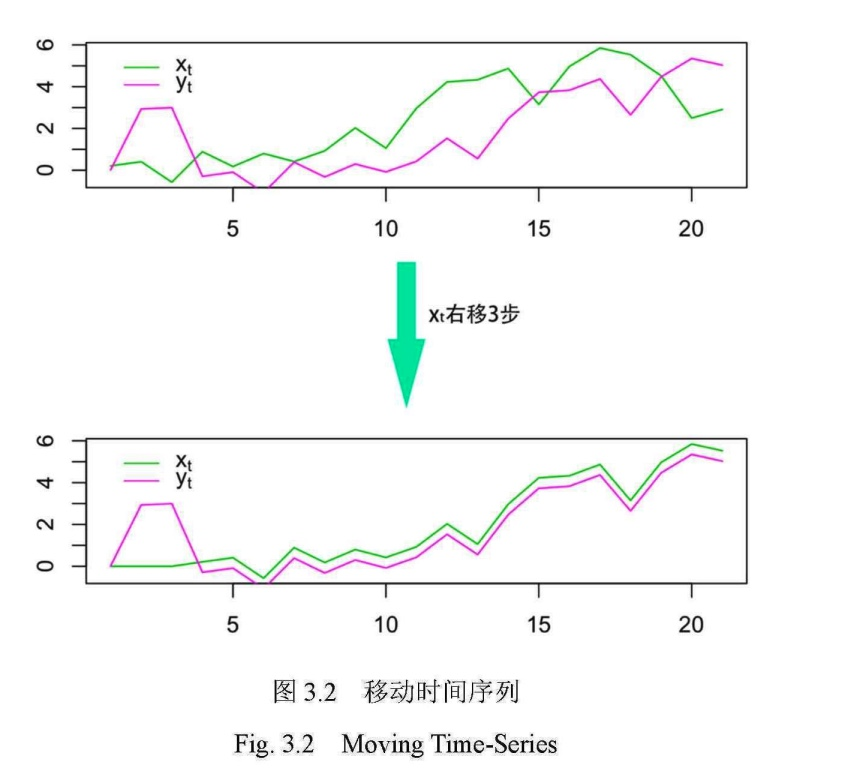
\includegraphics[scale=0.3,angle=0]{figure/NCC.jpg}\\
    \caption{移动时间序列}
    \label{fig:NCC}
\end{figure}
不同的时间序列数据可能在量级上差异巨大,需要对其归一化调整到相同的尺度。归一化是数据预处理中常用的技术,主要用于调整数据集中变量的尺度,使
其具有统一的标准。这通常通过将每个数据点减去平均值并除以标准差来实现,以便转化后的数据集具有零均值(\( \mu = 0 \))和单位方差
(\( \sigma^2 = 1 \))。这种转换被称为标准化或Z得分归一化。对于一个给定的时间序列 \( x_t \),其归一化后的值 \( x_t' \) 可以通过以下
公式计算得出:

\begin{equation}
x_t' = \frac{x_t - \mu}{\sigma}
\label{eq:normal1}
\end{equation}

其中,\( \mu \) 是原始时间序列 \( x_t \) 的均值,\( \sigma \) 是其标准差。这个过程确保了不同的数据集可以在相同的比例上进行比较和分析。K-Shape
算法采用系数归一化$NCC_c = \frac{CC_w(x,y)}{\|x\|\|y\|}$的方式对\( CC_w(x, y) \)进行归一化。互相关序列除以各个序列自的几何平均值。归一化后,
SBD的计算公式如式\eqref{eq:SBD}所示:
\begin{equation}
    SBD(x_t, y_t) = 1 - \max_w \left( \frac{CC_w(x_t, y_t)}{\|x_t\| \cdot \|y_t\|} \right)
    \label{eq:SBD}
\end{equation}
当两段时间序列重合越多,他们形状越相似,$CC_w(x_t, y_t)$就越大。对比所有可能位置的相似度值,取最相似的$max(NCC_c)$,再通过$1-max(NCC_c)$得到
SBD。表明了当两条时间序列越相似时,SBD越小。由于归一化以后的$NCC_c$在[-1,1]之间,因此SBD的值在[0,2]之间。当SBD=0时,意味着两条序列一模一样。
但是用上述方法对序列之间距离做对比时,时间复杂度为$O(m^2)$,当序列长度较长时,复杂度会很高,计算量也会很大。为解决这一问题,作者通过傅立叶变换的
方法,将序列从时域转换为频域再进行比较。此时,离散傅里叶变换(Discrete Fourier Transform, DFT)及其逆变换(Inverse Discrete Fourier Transform, IDFT)发挥了
至关重要的作用。DFT将时域信号转换为频域表示,而IDFT则实现了反向过程,允许序列从频域返回到时域。在K-shape聚类算法中,DFT和IDFT的运用可以描述如下。
给定时间序列 \( x_t \) 和 \( y_t \),首先应用DFT将这些序列转换为它们的频域表示 \( F(x_k) \) 和 \( F(y_k) \)。在频域中,通过简单地把原序列
的DFT结果,应用IDFT,我们可以有效地计算序列间在不同滑动窗口 \( w \) 下的互相关 \( CC_w(x_t, y_t) \)。
离散傅立叶变换和逆变换的数学表达式公式\eqref{eq:DFT}为:
\begin{equation}
    F(x_k) = \sum_{r=0}^{m-1} x_r e^{-\frac{2 \pi i r k}{m}}, \quad k = 0, \ldots, m - 1
    \label{eq:DFT}
\end{equation}
\begin{equation}
    F^{-1}(x_r) = \frac{1}{m} \sum_{k=0}^{m-1} F(x_k) e^{\frac{2 \pi i k r}{m}}, \quad r = 0, \ldots, m - 1
    \label{eq:IDFT}
\end{equation}
根据这些变换,互相关可以通过公式\eqref{eq:ccf}计算:
\begin{equation}
    CC_w(x_t, y_t) = F^{-1}(F(x_t) \times F(y_t))
    \label{eq:ccf}
\end{equation}
通过傅立叶变换的方式计算互相关的算法复杂度为\( O(m \log m) \),这使其计算SBD时在计算性能上十分高效,可以显著加快整个聚类过程。
K-Shape需要在簇内找到最优簇心$c_k^* = [c_1 \quad c_2 \quad \ldots \quad c_m]$使得簇$P_t$内所有序列$x_t$与$c_k^*$的SBD距离总和最小。其
等价的最大化问题为公式\eqref{eq:ck1}。
\begin{equation}
    c_k^* = \arg\min_{c_k} \sum_{x_t \in P_k} SBD(x_t, c_k)
    \label{eq:ck1}
\end{equation}
根据K-Shpae迭代的特性,将公式\eqref{eq:ck1}与公式\eqref{eq:SBD}结合,并将$c_k$标准化,可得到最终的簇心计算公式为式\eqref{eq:ckfin},其中$\mathbf{S} = \sum_{x_t \in P_k} x_t \cdot x_t^T$
\begin{equation}
    c_k^* = \arg\max_{c_k} \frac{c_k^T \cdot \mathbf{S} \cdot c_k}{c_k^T \cdot c_k}
    \label{eq:ckfin}
\end{equation}
此时,问题转化为了经典的瑞利商(Rayleigh Quotient)问题。只要求得矩阵$\mathbf{S}$的最大特征值,$c_k$的解就是$\mathbf{S}$最大特征值对应的特征向量。
\subsection{GRU}
\subsection{Transformer}